\section{Theoretical framework}
\label{sec: theory}

  Our attention is focused on the characterization of very high-dimensional nonlinear dynamical systems typically arising from the spatial discretization of partial differential equations such as the incompressible Navier-Stokes equations. In general, the resulting dynamical equations are written down as a system of first order differential equations
  \begin{equation}
    \dot{X}_j = \mathcal{F}_j \left( \left\{ X_i(t);\ i =1, \cdots, n \right\}, t \right)
    \notag
  \end{equation}
  where the integer $n$ is the \emph{dimension} of the system, and $\dot{X}_j$ denotes the time-derivative of $X_j$. Using the notation $\bf{X}$ and $\mathbfcal{F}$ for the sets $\left\{ X_j,\ i =1, \cdots, n \right\}$ and $\left\{ \mathcal{F}_j,\ i =1, \cdots, n \right\}$, this system can be compactly written as
  \begin{equation}
    \dot{\mathbf{X}} = \mathbfcal{F}(\mathbf{X}, t),
    \label{eq: theory -- continuous-time dynamical system}
  \end{equation}
  where $\mathbf{X}$ is the $n \times 1$ \emph{state vector} of the system and $t$ is a continuous variable denoting time. Alternatively, accounting also for temporal discretization gives rise to a discrete-time dynamical system
  \begin{equation}
    X_{j, k+1} = \mathcal{G}_j \left( \left\{ X_{i, k};\ i = 1, \cdots, n \right\}, k \right)
    \notag
  \end{equation}
  or formally
  \begin{equation}
    \mathbf{X}_{k+1} = \mathbfcal{G} \left( \mathbf{X}_k, k \right)
    \label{eq: theory -- discrete-time dynamical system}
  \end{equation}
  where the index $k$ now denotes the discrete time variable. If one uses first-order Euler extrapolation for the time discretization, the relation between $\mathbfcal{F}$ and $\mathbfcal{G}$ is given by
  \begin{equation}
    \mathbfcal{G} (\mathbf{X}) = \mathbf{X} + \Updelta t \mathbfcal{F}\left( \mathbf{X} \right),
    \notag
  \end{equation}
  where $\Updelta t$ is the time-step and the explicit dependences on $t$ and $k$ have been dropped for the sake of simplicity.

  In the rest of this section, the reader will be introduced to the concepts of fixed points and linear stability, two concepts required to characterize a number of properties of the system investigated. Particular attention will be paid to \emph{modal} and \emph{non-modal stability}, two approaches that have become increasingly popular in fluid dynamics over the past decades. Note that the concept of \emph{nonlinear optimal perturbation}, which has raised a lot attention lately, is beyond the scope of the present contribution. For interested readers, please refer to the recent work by \cite{nonlinear_optimal:kerswell:2014} and references therein.

  Finally, while we will mostly use the continuous-time representation \eqref{eq: theory -- continuous-time dynamical system} when introducing the reader to the theoretical concepts exposed in this section, using the discrete-time representation \eqref{eq: theory -- discrete-time dynamical system} will prove more useful when discussing and implementing the different algorithms presented in \textsection \ref{sec: numerics}.


  %%%%%%%%%%%%%%%%%%%%%%%%%%%%%%%%
  %%%%%                      %%%%%
  %%%%%     FIXED POINTS     %%%%%
  %%%%%                      %%%%%
  %%%%%%%%%%%%%%%%%%%%%%%%%%%%%%%%

  \subsection{Fixed points}
  \label{subsec: theory-fixed points}

  Nonlinear dynamical systems described by Eq.~\eqref{eq: theory -- continuous-time dynamical system} or Eq.~\eqref{eq: theory -- discrete-time dynamical system} tend to admit a number of different equilibria forming the backbone of their phase space. These different equilibria can take the form of fixed points, periodic orbits, torus or strange attractors for instance. In the rest of this work, our attention will be solely focused on fixed points.

  For a continuous-time dynamical system described by Eq.~\eqref{eq: theory -- continuous-time dynamical system}, fixed points $\mathbf{X}^{*}$ are solution to
  \begin{equation}
    \mathbfcal{F}\left( \mathbf{X} \right) = 0.
    \label{eq: theory -- continuous-time fixed point}
  \end{equation}
  Conversely, fixed points $\mathbf{X}^*$ of a discrete-time dynamical system described by Eq.~\eqref{eq: theory -- discrete-time dynamical system} are solution to
  \begin{equation}
    \mathbfcal{G} \left( \mathbf{X} \right) = \mathbf{X}.
    \label{eq: theory -- discrete-time fixed point}
  \end{equation}
  It must be emphasized that both Eq.~\eqref{eq: theory -- continuous-time fixed point} and Eq.~\eqref{eq: theory -- discrete-time fixed point} may admit multiple solutions. Such a multiplicity of fixed points can easily be illustrated by a dynamical system as simple as the following Duffing oscillator
  \begin{equation}
    \begin{aligned}
      \dot{x} & = y \\
      \dot{y} & = -\displaystyle \frac{1}{2} y + x - x^3.
    \end{aligned}
    \label{eq: theory -- Duffing oscillator}
  \end{equation}
  Despite its apparent simplicity, this Duffing oscillator admits three fixed points, namely
  \begin{itemize}
    \item a saddle at the origin $\mathbf{X}^* = (0, 0)$,
    \item two linearly stable spirals located at $\mathbf{X}^* = (\pm 1, 0)$.
  \end{itemize}
  All of these fixed points, along with some trajectories, are depicted on figure \ref{fig: theory -- Duffing oscillator} for the sake of illustration. Such a multiplicity of fixed points also occurs in dynamical systems as complex as the Navier-Stokes equations. Determining which of these fixed points is the most relevant one from a physical point of view is problem-dependent and left for the user to decide. Note however that computing these equilibrium points is a prerequisite to all of the analyses to be described in this chapter. Numerical methods to solve Eq.~\eqref{eq: theory -- continuous-time fixed point} or Eq.~\eqref{eq: theory -- discrete-time fixed point} will be discussed in \textsection \ref{subsec: numerics-fixed points computation}.

  \begin{figure}[b]
    \centering
    \sidecaption
    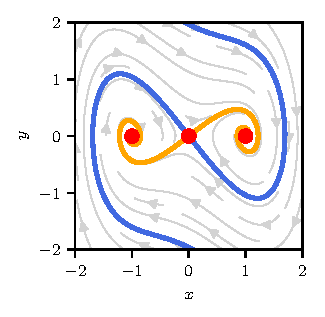
\includegraphics[scale=1]{duffing_oscillator_saddle_manifold}
    \caption{Phase portrait of the unforced Duffing oscillator \eqref{eq: theory -- Duffing oscillator}. The red dots denote the three fixed points admitted by the system. The blue (resp. orange) thick line depicts the stable (resp. unstable) manifold of the saddle point located at the origin. Grey lines highlight a few trajectories exhibited for different initial conditions.}
    \label{fig: theory -- Duffing oscillator}
  \end{figure}

  %%%%%%%%%%%%%%%%%%%%%%%%%%%%%%%%%%%%
  %%%%%                          %%%%%
  %%%%%     LINEAR STABILITY     %%%%%
  %%%%%                          %%%%%
  %%%%%%%%%%%%%%%%%%%%%%%%%%%%%%%%%%%%

  \subsection{Linear stability analysis}
  \label{subsec: theory -- linear stability}

  Having computed a given fixed point $\mathbf{X}^*$ of a continuous-time nonlinear dynamical system given by Eq. \eqref{eq: theory -- continuous-time dynamical system}, one may ask whether it corresponds to a stable or unstable equilibrium of the system. Before pursuing, the very notion of \emph{stability} needs to be explained. It is traditionally defined following the concept of Lyapunov stability. Having computed the equilibrium state $\mathbf{X}^*$, the system is perturbed around this state. If it returns back to the equilibrium point, the latter is deemed stable, otherwise, it is regarded as unstable. It has to be noted that, in the concept of Lyapunov stability, an infinite time horizon is allowed for the return to equilibrium.

  The dynamics of a perturbation $\mathbf{x} = \mathbf{X} - \mathbf{X}^*$ are governed by
  \begin{equation}
    \dot{\mathbf{x}} = \mathbfcal{F}(\mathbf{X}^* + \mathbf{x}).
  \end{equation}
  Assuming the perturbation $\mathbf{x}$ is infinitesimal, $\mathbfcal{F}(\mathbf{X})$ can be approximated by its first-order Taylor expansion around $\mathbf{X} = \mathbf{X}^*$. Doing so, the governing equations for the perturbation $\mathbf{x}$ simplify to
  \begin{equation}
    \dot{\mathbf{x}} = \mathbfcal{A}\mathbf{x},
    \label{eq: theory -- linear perturbation dynamics}
  \end{equation}
  where $\mathbfcal{A}$ is the $n \times n$ Jacobian matrix of $\mathbfcal{F}$. Starting from an initial condition $\mathbf{x}_0$, the perturbation at time $t$ is given by
  \begin{equation}
    \mathbf{x}(t) = \exp \left( \mathbfcal{A}t \right) \mathbf{x}_0.
    \label{eq: theory -- linear stability solution}
  \end{equation}
  The operator $\mathbfcal{M}(t) = \exp \left( \mathbfcal{A}t \right)$ is known as the \emph{exponential propagator}. Introducing the spectral decomposition of $\mathbfcal{A}$
  \begin{equation}
    \mathbfcal{A} = \mathbfcal{V} \boldsymbol{\Lambda} \mathbfcal{V}^{-1},
    \notag
  \end{equation}
  Eq. \eqref{eq: theory -- linear stability solution} can be rewritten as
  \begin{equation}
    \mathbf{x}(t) = \mathbfcal{V} \exp \left( \boldsymbol{\Lambda} t \right) \mathbfcal{V}^{-1} \mathbf{x}_0,
  \end{equation}
  where the i\textsuperscript{th} column of $\mathbfcal{V}$ is the eigenvector $\mathbf{v}_i$ associated to the i\textsuperscript{th} eigenvalue $\lambda_i = \boldsymbol{\Lambda}_{ii}$, with $\boldsymbol{\Lambda}$ a diagonal matrix. Assuming that the eigenvalues of $\mathbfcal{A}$ have been sorted by decreasing real part, it can easily be shown that
  \begin{equation}
    \lim\limits_{t \to + \infty} \exp \left( \mathbfcal{A} t \right) \mathbf{x}_0 = \lim \limits_{t \to + \infty} \exp \left( \lambda_1 t \right) \mathbf{v}_1 .
    \notag
  \end{equation}
  The asymptotic fate of an initial perturbation $\mathbf{x}_0$ is thus entirely dictated by the real part of the leading eigenvalue $\lambda_1$:
  \begin{itemize}
    \item if $\Re \left( \lambda_1 \right) > 0$, a random initial perturbation $\mathbf{x}_0$ will eventually grow exponentially rapidly. Hence, the fixed point $\mathbf{X}^*$ is deemed \emph{linearly unstable}.

    \item If $\Re \left( \lambda_1 \right) < 0$, the initial perturbation $\mathbf{x}_0$ will eventually decay exponentially rapidly. The fixed point $\mathbf{X}^*$ is thus \emph{linearly stable}.
  \end{itemize}
  The case $\Re \left( \lambda_1 \right) = 0$ is peculiar. The fixed point $\mathbf{X}^*$ is called \emph{elliptic} and one cannot conclude about its stability solely by looking at the eigenvalues of $\mathbfcal{A}$. In this case, one needs to resort to \emph{weakly non-linear analysis} which essentially looks at the properties of higher-order Taylor expansion of $\mathbfcal{F} \left( \mathbf{X} \right)$. Once again, this is beyond the scope of the present chapter. Interested readers are referred to \cite{??} for more details about such analyses.

  \paragraph*{Illustration}

  Let us illustrate the notion of linear stability on a simple example. For that purpose, we will consider the same linear dynamical system as in \cite{amr:schmid:2014}. This system reads
  \begin{equation}
    \displaystyle \frac{\mathrm{d}}{\mathrm{d}t} \begin{bmatrix} x_1 \\ x_2 \end{bmatrix} =
    \underbrace{
    \begin{bmatrix}
      \displaystyle \frac{1}{100} - \frac{1}{Re} & 0 \\
      1 & \displaystyle -\frac{2}{Re}
    \end{bmatrix}
    }_{\mathbfcal{A}}
    \begin{bmatrix} x_1 \\ x_2 \end{bmatrix}
    \label{eq: theory -- schmid system}
  \end{equation}
  where $Re$ is a control parameter. For such a simple case, it is obvious that the eigenvalues of $\mathbfcal{A}$ are given by
  \begin{equation}
    \lambda_1 = \displaystyle \frac{1}{100} - \frac{1}{Re}
    \notag
  \end{equation}
  and
  \begin{equation}
    \lambda_2 = - \frac{2}{Re}.
    \notag
  \end{equation}
  While $\lambda_2$ is constantly negative, $\lambda_1$ is negative for $Re < 100$ and positive otherwise. Figure \ref{fig: theory -- illustration modal stability} depicts the time-evolution of $\| \mathbf{x} \|_2^2 = x_1^2 + x_2^2$ for two different values of $Re$. Please note that the short-time ($t < 100$) behavior of the perturbation will be discussed in \textsection \ref{subsec: theory -- non-modal stability}. It is clear nonetheless that, for $t>100$, the time-evolution of the perturbation can be described by an exponential function. Whether this exponential increases or decreases as a function of time is solely dictated by the sign of $\lambda_1$, negative for $Re=50$ and positive for $Re=100$. For $Re=50$, the equilibrium point $\mathbf{X}^* = \begin{bmatrix} 0 & 0 \end{bmatrix}^T$ is thus stable, while it is unstable for $Re=125$.

  \begin{figure}[b]
    \centering
    \sidecaption
    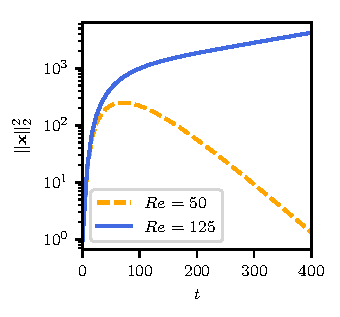
\includegraphics[scale=1]{S2_Theory_illustration_linear_stability}
    \caption{Evolution as a function of time of $\| \mathbf{x} \|_2^2 = x_1^2 + x_2^2$ for the toy-model \eqref{eq: theory -- schmid system}. For $Re=50$ (resp. $Re=125$), the asymptotic fate of $\| \mathbf{x} \|_2^2$ is described by a decreasing (resp. increasing) exponential. For $Re=50$, the equilibrium point is thus linear stable, while it is linearly unstable for $Re=125$.}
    \label{fig: theory -- illustration modal stability}
  \end{figure}

  %%%%%%%%%%%%%%%%%%%%%%%%%%%%%%%%%%%%%%%%%%%%%%%%
  %%%%%                                      %%%%%
  %%%%%     NON-MODAL STABILITY ANALYSIS     %%%%%
  %%%%%                                      %%%%%
  %%%%%%%%%%%%%%%%%%%%%%%%%%%%%%%%%%%%%%%%%%%%%%%%

  \subsection{Non-modal stability analysis}
  \label{subsec: theory -- non-modal stability}

  Looking once more at figure \ref{fig: theory -- illustration modal stability}, it can be seen that, although the system is linearly stable for $Re=50$, the perturbation $\mathbf{x}$ can experience a transient growth of its energy for a short period of time, roughly given by $0 < t <100$ in the present case, before its eventual exponential decay. This behavior is related to the \emph{non-normality} of $\mathbfcal{A}$, i.e.\
  \begin{equation}
    \mathbfcal{A}^{\dagger} \mathbfcal{A} \neq \mathbfcal{A} \mathbfcal{A}^{\dagger},
    \label{eq: theory -- non-normality equation}
  \end{equation}
  where $\mathbfcal{A}^{\dagger}$ is the \emph{adjoint} of $\mathbfcal{A}$. As a result of this non-normality, the eigenvectors of $\mathbfcal{A}$ do not form an orthonormal set of vectors\footnote{Note that the non-normality of $\mathbfcal{A}$ also implies that its right and left eigenvectors are different. As will be discussed in \textsection \ref{sec: application}, this observation may have large consequences in fluid dynamics, particularly when addressing the problems of optimal linear control and/or estimation of strongly non-parallel flows.}. The consequences of this non-orthogonality of the set of eigenvectors can be visualized on figure \ref{fig: theory -- illustration transient growth} where the trajectory stemming from a random unit-norm initial condition $\mathbf{x}_0$ is depicted in the phase plane of our toy-model \eqref{eq: theory -- schmid system}. The perturbation $\mathbf{x}(t)$ is first attracted toward the linear manifold associated to the least stable eigenvalue $\lambda_1$, causing in the process the transient growth of its energy by a factor 300. Once it reaches the vicinity of the linearly stable manifold, the perturbation eventually decays exponentially rapidly along this eigendirection of the fixed point. The next sections are devoted to the introduction of mathematical tools particularly useful to characterize phenomena resulting from this non-normality of $\mathbfcal{A}$, both in the time and frequency domains, when the fixed point considered is stable.

  \begin{figure}[b]
    \centering
    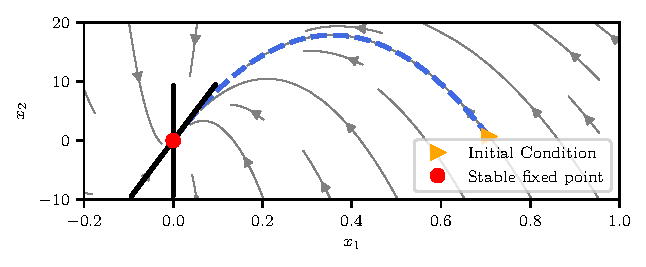
\includegraphics[scale=1]{S2_Theory_explanation_transient_growth}
    \caption{The blue (dashed) line shows the trajectory stemming from a random unit-norm initial condition $\mathbf{x}_0$. The thick black lines depict the two linear manifolds of the fixed point. The diagonal one corresponds to $\lambda_1 = \nicefrac{1}{100} - \nicefrac{1}{Re}$, while the vertical one is associated to $\lambda_2 = -\nicefrac{2}{Re}$. In the present case, $Re$ is set to 50, thus corresponding to a situation where the fixed point is linearly stable. Note that different scales are used for the horizontal and vertical axes.}
    \label{fig: theory -- illustration transient growth}
  \end{figure}

    %-----> Optimal perturbation.
    \subsubsection{Optimal perturbation analysis}
    \label{subsubsec: theory -- optimal perturbation}

    Having observed that a random initial condition can experience a relatively large transient growth of its energy over a short period of time even though the fixed point is stable, one may be interested in the worst case scenario, i.e.\ finding which initial condition $\mathbf{x}_0$ is amplified as much as possible before it eventually decays. Searching for such a perturbation is known as \emph{optimal perturbation analysis} and can be addressed by two different methods:
    \begin{itemize}
      \item Optimization,
      \item Singular Value Decomposition (SVD).
    \end{itemize}
    Both approaches will be presented. Although it requires the introduction of additional mathematical concepts, the approach relying on optimization will be introduced first in \textsection \ref{paragraph: theory -- optimal perturbation optimization} as it easier to grasp. The approach relying on singular value decomposition of the exponential propagrator $\mathbfcal{M} = \exp \left( \mathbfcal{A} t \right)$ will then be presented in \textsection \ref{paragraph: theory -- optimal perturbation svd}.

      % --> Lagrange multipliers.
      \paragraph{Formulation as an optimization problem}
      \label{paragraph: theory -- optimal perturbation optimization}

      The aim of optimal perturbation analysis is to find the unit-norm initial condition $\mathbf{x}_0$ that maximizes $\| \mathbf{x}(T) \|_2^2$, where $T$ is known as the \emph{target time}. Note that we here consider only the 2-norm of $\mathbf{x}(T)$ for the sake of simplicity, although one could formally optimize different norms, see \cite{??} for examples from fluid dynamics. For a given target time $T$, such a problem can be formulated as the following constrained maximization problem
      \begin{equation}
          \begin{aligned}
            \maximize \limits_{\mathbf{x}_0} & \mathcal{J} \left( \mathbf{x}_0 \right) = \| \mathbf{x}(T) \|_2^2\\
            \subjecto & \dot{\mathbf{x}} - \mathbfcal{A}\mathbf{x} = 0 \\
            ~ & \| \mathbf{x}_0 \|_2^2 - 1 = 0,
          \end{aligned}
          \label{eq: theory -- constrained maximization}
      \end{equation}
      where $\mathcal{J}(\mathbf{x}_{0})$ is known as the \emph{objective function}. It must be emphasized that problem \eqref{eq: theory -- constrained maximization} is not formulated as a convex optimization problem\footnote{
      Formally, a convex optimization problem reads
      \begin{equation}
        \begin{aligned}
          \minimize \limits_{\mathbf{x}} & \mathcal{J} \left( \mathbf{x} \right) \\
          \subjecto & g_i \left( \mathbf{x} \right) \leq 0, \ i = 1, \cdots, m \\
          ~ & h_i \left( \mathbf{x} \right) = 0, \ i = 1, \cdots, p,
        \end{aligned}
        \notag
      \end{equation}
      where the objective function $\mathcal{J} \left( \mathbf{x} \right)$ and the inequality constraints functions $g_i \left( \mathbf{x} \right)$ are convex. The conditions on the equality constraints functions $h_i \left( \mathbf{x} \right)$ are more restrictive as they need to be affine functions, i.e.\ of the form $h_i \left( \mathbf{x} \right) = \mathbf{a}_i^T \mathbf{x} + b_i$. See the book by Boyd \& Vandenberghe \cite{book:boyd:2004} for extensive details about convex optimization.}.
      As such, it may exhibit local maxima. Nonetheless, this constrained maximization problem can be recast into the following unconstrained maximization problem
      \begin{equation}
        \maximize \limits_{\mathbf{x}, \mathbf{v}, \mu} \mathcal{L} \left( \mathbf{x}, \mathbf{v}, \mu \right),
        \label{eq: theory -- unconstrained maximization}
      \end{equation}
      where
      \begin{equation}
        \mathcal{L} \left( \mathbf{x}, \mathbf{v}, \mu \right) = \mathcal{J}\left( \mathbf{x}_0 \right) + \int_{0}^T \mathbf{v}^T \left( \dot{\mathbf{x}} - \mathbfcal{A}\mathbf{x} \right) \mathrm{d}t + \mu \left( \| \mathbf{x}_0 \|_2^2 - 1 \right)
        \label{eq: theory -- augmented Lagrangian}
      \end{equation}
      is known as the \emph{augmented Lagrangian} function. The additional optimization variables $\mathbf{v}$ and $\mu$ appearing in the definition of the augmented Lagrangian $\mathcal{L}$ are called \emph{Lagrange multipliers}. Solutions to problem \eqref{eq: theory -- unconstrained maximization} are identified by vanishing first variations of $\mathcal{L}$ with respect to our three optimization variables. The first variation of $\mathcal{L}$ with respect to $\mathbf{v}$ and $\mu$ are simply the constraints of our original problem \eqref{eq: theory -- constrained maximization}. The first variation of $\mathcal{L}$ with respect to $\mathbf{x}$ on the other hand is given by
      \begin{equation}
        \delta_{\mathbf{x}} \mathcal{L} = \left[ \nabla_{\mathbf{x}} \mathcal{J} + \mathbf{v}(T) \right] \cdot \delta \mathbf{x}(0) + \int_0^T \left[ \dot{\mathbf{v}} - \mathbfcal{A}^{\dagger} \mathbf{v} \right] \cdot \delta \mathbf{x} \ \mathrm{dt} + \left[ 2\mu \mathbf{x}_0 - \mathbf{v}(0) \right] \cdot \delta \mathbf{x}(0).
        \label{eq: theory -- optimality condition}
      \end{equation}
      Eq. \eqref{eq: theory -- optimality condition} vanishes only if
      \begin{equation}
        \dot{\mathbf{v}} = \mathbfcal{A}^{\dagger} \mathbf{v} \ \text{ over } t \in \left( 0, T \right),
        \label{eq: theory -- adjoint equations}
      \end{equation}
      and
      \begin{equation}
        \begin{aligned}
          \nabla_{\mathbf{x}} \mathcal{J} - \mathbf{v}(T) & = 0 \\
          2\mu \mathbf{x}_0 - \mathbf{v}(0) & = 0.
        \end{aligned}
        \label{eq: theory -- compatibility conditions}
      \end{equation}
      Note that Eq. \eqref{eq: theory -- adjoint equations} is known as the adjoint system\footnote{
      Given an appropriate inner product, the adjoint operator $\mathbfcal{A}^{\dagger}$ is defined such that
      \begin{equation}
        \langle \mathbf{v} \vert \mathbfcal{A} \mathbf{x} \rangle = \langle \mathbfcal{A}^{\dagger} \mathbf{v} \vert \mathbf{x} \rangle,
        \notag
      \end{equation}
      where $\langle \mathbf{a} \vert \mathbf{b} \rangle$ denotes the inner product of $\mathbf{a}$ and $\mathbf{b}$. If one consider the classical Euclidean inner product, the adjoint operator is simply given by
      $$\mathbfcal{A}^{\dagger} = \mathbfcal{A}^H$$
      where $\mathbfcal{A}^H$ is the Hermitian (i.e.\ complex-conjugate transpose) of $\mathbfcal{A}$. It must be noted finally that the direct operator $\mathbfcal{A}$ and the adjoint one $\mathbfcal{A}^{\dagger}$ have the same eigenspectrum. This last observation is a key point when one aims at validating the numerical implementation of an adjoint solver.
      }
      of our original linear dynamical system, while Eq. \eqref{eq: theory -- compatibility conditions} are called compatibility conditions. Maximizing $\mathcal{L}$ is then a problem of simultaneously satisfying \eqref{eq: theory -- linear perturbation dynamics}, \eqref{eq: theory -- adjoint equations} and \eqref{eq: theory -- compatibility conditions}. This is in general done iteratively by gradient-based algorithms such as gradient ascent or the rotation-update gradient algorithm (see \textsection \ref{sec: numerics}). For more details about adjoint-based optimization, see \cite{book:boyd:2004, nonlinear_optimal:kerswell:2014}.

      %--> A Rayleigh quotient problem.
      \paragraph{Formulation using SVD}
      \label{paragraph: theory -- optimal perturbation svd}

      As stated previously, formulating the optimal perturbation analysis as a constrained maximization results in a non-convex optimization problem \eqref{eq: theory -- constrained maximization}. Consequently, although a solution to \eqref{eq: theory -- constrained maximization} can easily be obtained by means of gradient-based algorithms, one cannot rule out the possibility that this solution is only a local maxima rather than the global one. In this section, we will show that recasting problem \eqref{eq: theory -- constrained maximization} in the framework of linear algebra however allows us to obtain easily this global optimal.

      Let us first redefine our optimization problem as
      \begin{equation}
        \maximize_{\mathbf{x}_0} \displaystyle \frac{\| \mathbf{x}(T) \|_2^2}{\| \mathbf{x}_0 \|_2^2}
        \label{eq: theory -- energy gain}
      \end{equation}
      so that rather than maximizing $\| \mathbf{x}(T) \|_2^2$ under the constraint that $\| \mathbf{x}_0 \|_2^2 = 1$, we now directly aim to maximize the energy gain $\mathcal{G}(T) = \nicefrac{\| \mathbf{x}(T) \|_2^2}{\| \mathbf{x}_0 \|_2^2}$. Moreover, recalling from \eqref{eq: theory -- linear stability solution} that
      \begin{equation}
        \mathbf{x}(T) = \exp \left( \mathbfcal{A} T \right) \mathbf{x}_0,
        \notag
      \end{equation}
      our energy gain maximization problem can finally be written as
      \begin{equation}
        \begin{aligned}
          \mathcal{G}(T) & = \max_{\mathbf{x}_0} \displaystyle \frac{\| \exp \left( \mathbfcal{A} t \right) \mathbf{x}_0 \|_2^2}{\| \mathbf{x}_0 \|_2^2} \\
          & = \| \exp \left( \mathbfcal{A} T \right) \|_2^2
        \end{aligned}
      \end{equation}
      where $\| \exp \left( \mathbfcal{A} T \right) \|_2$ is a vector-induced matrix norm taking care of the optimization over all possible initial conditions $\mathbf{x}_0$. Introducing singular value decomposition (SVD), i.e.\
      \begin{equation}
        \mathbfcal{M} = \mathbfcal{U} \boldsymbol{\Sigma} \mathbfcal{V}^H,
        \notag
      \end{equation}
      it is relatively easy to demonstrate that the optimal energy gain $\mathcal{G}(T)$ is given by
      \begin{equation}
        \mathcal{G}(T) = \sigma_1^2,
        \label{theory -- optimal energy gain }
      \end{equation}
      where $\sigma_1$ is the largest singular value of the exponential propagator $\mathbfcal{M} = \exp \left( \mathbfcal{A} T \right)$. The optimal initial condition $\mathbf{x}_0$ is then given by the principal right singular vector (i.e.\ $\mathbf{x}_0 = \mathbf{v}_1$), while the associated response is given by $\mathbf{x}(T) = \sigma_1 \mathbf{u}_1$, where $\mathbf{u}_1$ is the principal left singular vector.

      % --> Illustration.
      \paragraph{Illustration}

      As to illustrate linear optimal perturbations, let us consider the incompressible flow of a Newtonian fluid induced by two flat plates moving in-plane in opposite directions as sketched on figure \ref{fig: theory -- optimal perturbation illustration}(a). The resulting flow, known as \emph{plane Couette flow}, is given by
      $$U(y) = y.$$
      Note that it is a linearly stable fixed point of the Navier-Stokes equations no matter the Reynolds number considered. Despite its linear stability, subcritical transition to turbulence can occur for Reynolds numbers as low as $Re=??$.

      Without getting to deep into the mathematical and physical details of such subcritical transition, part of the explanation can be given by linear optimal perturbation analysis. The dynamics of an infinitesimal perturbation $\mathbf{x} = \begin{bmatrix} \mathbf{v} & \mathbf{\eta} \end{bmatrix}^T$, characterized by a certain wavenumber $\mathbf{k} = \alpha \mathbf{e}_x + \beta \mathbf{e}_z$, evolving in the vicinity of this fixed point are governed by
      \begin{equation}
        \displaystyle \frac{\mathrm{d}}{\mathrm{d}t} \begin{bmatrix} \mathbf{v} \\ \mathbf{\eta} \end{bmatrix} = \begin{bmatrix} \mathbfcal{A}_{OS} & 0 \\ \mathbfcal{C} & \mathbfcal{A}_{S} \end{bmatrix} \begin{bmatrix} \mathbf{v} \\ \mathbf{\eta} \end{bmatrix}
        \label{eq: theory -- orr-sommerfeld-squire equations}
      \end{equation}
      where $\mathbf{v}$ is the wall-normal velocity of the perturbation and $\mathbf{\eta}$ its wall-normal vorticity, $\mathbfcal{A}_{OS}$ is the Orr-Sommerfeld operator, while $\mathbfcal{A}_{S}$ is the Squire one. The operator $\mathbfcal{C}$ describes the existing coupling between the wall-normal velocity $\mathbf{v}$ and the wall-normal vorticity $\mathbf{\eta}$. For certain pairs of wavenumbers, this Orr-Sommerfeld-Squire operator is highly non-normal and perturbations can exhibit very large transient growth. This is illustrated on figure \ref{fig: theory -- optimal perturbation illustration}(a) where the evolution of the optimal gain $\mathcal{G}(T)$ as a function of the target time $T$ is depicted for different pairs of wavenumbers $(\alpha, \beta)$. The maximum amplification achievable over all target times $T$ and wavenumbers pairs $(\alpha, \beta)$ is $\mathcal{G}_{\mathrm{opt}} \simeq 100$. The initial perturbation $\mathbf{x}_0$ corresponding to this optimal energy gain is depicted on figure \ref{fig: theory -- optimal perturbation illustration}(b). It corresponds to streamwise-oriented vortices that eventually give rise to streamwise velocity streaks due to the lift-up effect \cite{jfm:landahl:1980, ejmbf:brandt:2014}, see figure \ref{fig: theory -- optimal perturbation illustration}(d). While this perturbation eventually decays exponentially rapidly in a purely linear framework, it has been shown that, for a sufficiently large initial amplitude, it may eventually trigger transition to turbulence when used as initial condition in a non-linear direct numerical simulation of the Navier-Stokes equations \cite{??}. For more details about subcritical transition and extension of optimal perturbation analysis to non-linear operators, interested readers are referred to \cite{??}.

      \begin{figure}[b]
        \centering
        \subfigure[]{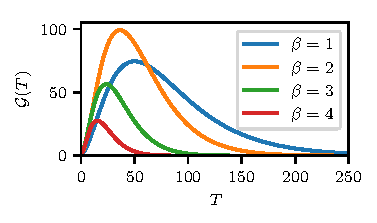
\includegraphics[scale=1]{S2_optimal_perturbation_couette_flow_gain}} \\
        \subfigure[]{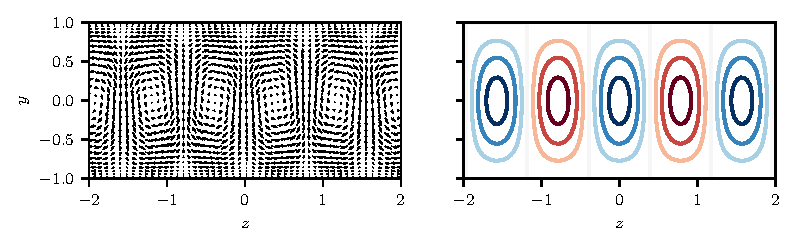
\includegraphics[scale=1]{S2_optimal_perturbation_couette_flow}}
        \caption{Illustration of optimal perturbation analysis for the plane Couette flow at $Re=300$. In all cases, the streamwise wavenumber of the perturbation is set to $\alpha=0$. (a) Optimal gain curve for different spanwise wavenumbers $\beta$. (b) Optimal perturbation (left) and optimal response (right) for $\beta=2$. Note that optimal perturbation consists of streamwise oriented vortices, while the associated response at time $T$ consist in high- and low-speed streaks.}
        \label{fig: theory -- optimal perturbation illustration}
      \end{figure}

    \subsubsection{Resolvent analysis}
    \label{subsubsec: theory -- resolvent perturbation}

    The optimal perturbation analysis (see \textsection \ref{subsubsec: theory -- optimal perturbation}) aims at finding the initial condition $\mathbf{x}_0$ that maximizes the transient amplification of energy of the response $\mathbf{x}(T) = \exp \left( \mathbfcal{A} T \right) \mathbf{x}_0$ at the target time $t=T$. It is thus an initial-value problem that can be investigated in the time domain. Rather than considering the response of the system to different initial conditions, one may instead wonder how the system reacts to external noise. For that purpose, let us now consider a forced linear dynamical system
    \begin{equation}
      \dot{\mathbf{x}} = \mathbfcal{A} \mathbf{x} + \mathbf{f}
      \label{eq: theory -- forced linear system}
    \end{equation}
    where the forcing $\mathbf{f}$ now models the system's input such as the external noise. As before, we moreover assume that all of the eigenvalues of $\mathbfcal{A}$ lie within the stable half of the complex plane. As for the optimal perturbation analysis, one may now consider a worst-case scenario, i.e.\ what is the forcing $\mathbf{f}$ that maximizes the asymptotic response of the system? Because we consider a linear dynamical system, this question can naturally be addressed in the frequency domain.

    In the most general case, the response of the system to the forcing $\mathbf{f}(t)$ is given by
    \begin{equation}
      \mathbf{x}(t) = \int_0^t \exp \left( \mathbfcal{A} (t-\tau) \right) \mathbf{f}(\tau) \ \mathrm{d}\tau
      \label{eq: theory -- convolution integral}
    \end{equation}
    which is a convolution integral. Note that, in the above expression, we assumed a zero initial condition, i.e.\ $\mathbf{x}_0 = 0$. Such a convolution integral is also known as a memory integral and highlights that the current state $\mathbf{x}(t)$ of the system depends on the entire history of the forcing $\mathbf{f}$. Because we consider linear stable systems, the influence of the forcing on the current state decays exponentially according to the least stable eigenvalue. Let us assume furthermore a harmonic external forcing
    \begin{equation}
      \mathbf{f}(t) = \Re \left( \hat{\mathbf{f}} e^{i \omega t} \right)
    \end{equation}
    where $\omega \in \mathbb{R}$ is the circular frequency of the forcing. The convolution integral can now be easily computed in the frequency domain. Given our assumptions, the asymptotic response of the system at the frequency $\omega$ is given by
    \begin{equation}
      \hat{\mathbf{x}} = \left( i \omega \mathbfcal{I} - \mathbfcal{A} \right)^{-1} \hat{\mathbf{f}}.
      \label{eq: theory -- transfer function}
    \end{equation}
    The operator $\mathbfcal{R}(\omega) = \left( i \omega \mathbfcal{I} - \mathbfcal{A} \right)^{-1}$ appearing in Eq. \eqref{eq: theory -- transfer function} is known as the \emph{Resolvent operator} and is related to the exponential propagator $\mathbfcal{M}(t) = \exp \left( \mathbfcal{A} t \right)$ via Laplace transform. This operator, acting in the frequency domain, maps the input harmonic forcing $\hat{\mathbf{f}}(\omega)$ to the output harmonic response $\hat{\mathbf{x}}(\omega)$.

    Finding the forcing frequency $\omega$ that maximizes the asymptotic response $\mathbf{x}$ of the system can now be formalized as
    \begin{equation}
      \begin{aligned}
        \mathcal{R}(\omega) & = \max_{\hat{\mathbf{f}}} \displaystyle \frac{\| \left( i \omega \mathbfcal{I} - \mathbfcal{A} \right)^{-1} \hat{\mathbf{f}} \|_2^2}{\| \hat{\mathbf{f}} \|_2^2} \\
        & = \| \mathbfcal{R}(\omega) \|_2^2.
      \end{aligned}
      \label{eq: theory -- resolvent norm}
    \end{equation}
    Going from the time domain to the frequency domain, the norm of the exponential propagator is replaced with that of the resolvent in order quantify the energy amplification between the input forcing and the output response. As before, the optimal resolvent gain at the frequency $\omega$ is given by
    \begin{equation}
      \mathcal{R}(\omega) = \sigma_1^2,
      \notag
    \end{equation}
    where $\sigma_1$ is the largest singular value of $\mathbfcal{R}(\omega)$. The associated optimal forcing $\hat{\mathbf{f}}$ and response $\hat{\mathbf{x}}$ are then given by the corresponding right and left singular vectors, respectively.

    % --> Illustration.
    \paragraph{Illustration}

    Once more, let us illustrate the use of the resolvent analysis on an example from fluid dynamics. For that purpose, we will consider an axisymmetric jet whose radial velocity profile is given by
    \begin{equation}
      U(r) = ??.
      \label{eq: theory -- resolvent analysis - jet profile}
    \end{equation}

    {\color{red} I need to run this whole analysis to write down this part.}
